\providecommand{\main}{../..}
\documentclass[\main/dresen_thesis.tex]{subfiles}

\begin{document}
\chapter{Loosely-packed nanostructures}\label{ch:looselyPackedNS}
Magnetic nanospheres can nowadays be routinely synthesized from a large choice of materials \cite{Gubin_2005_Magne}.
Due to it's strong ferromagnetic properties and wide availability, iron oxide is a common choice for the study of nanomagnetism.
Due to this extensive research it is now possible to synthesize iron oxide nanoparticles that are highly tunable in size and shape \cite{Wetterskog_2014_Preci}.
In this work, two batches of iron oxide nanospheres in the size range of $10 \unit{nm}$ and $7 \unit{nm}$ were studied for their individual structural and magnetic properties.
Furthermore, loosely packed layers of the nanoparticles, created by spin coating the particles from dispersion on a substrate, were studied.
The magnetic properties of the nanostructure are compared to the individual nanoparticle properties and compared to model calculations to search for emergent effects arising from dipolar interparticle interaction.

\section{Spherical iron oxide nanoparticles}
Iron oxide nanoparticles were obtained from a collaboration with the group of Prof. Tremel from the inorganic chemistry department of the university of Mainz.
Briefly, they were prepared by following a popular synthesis route where first iron oleate is prepared from iron(III) chloride and then nanospheres are obtained by a controlled thermal decomposition of the oleate at high temperatures.
A similar synthesis route procedure is used later in this work for the preparation of cobalt iron oxide nanocubes and is explained in more detail in \refsec{ch:monolayers}.

In a first step, the iron oxide nanospheres are characterized by transmission electron microscopy.
\begin{figure}[tb]
  \centering
  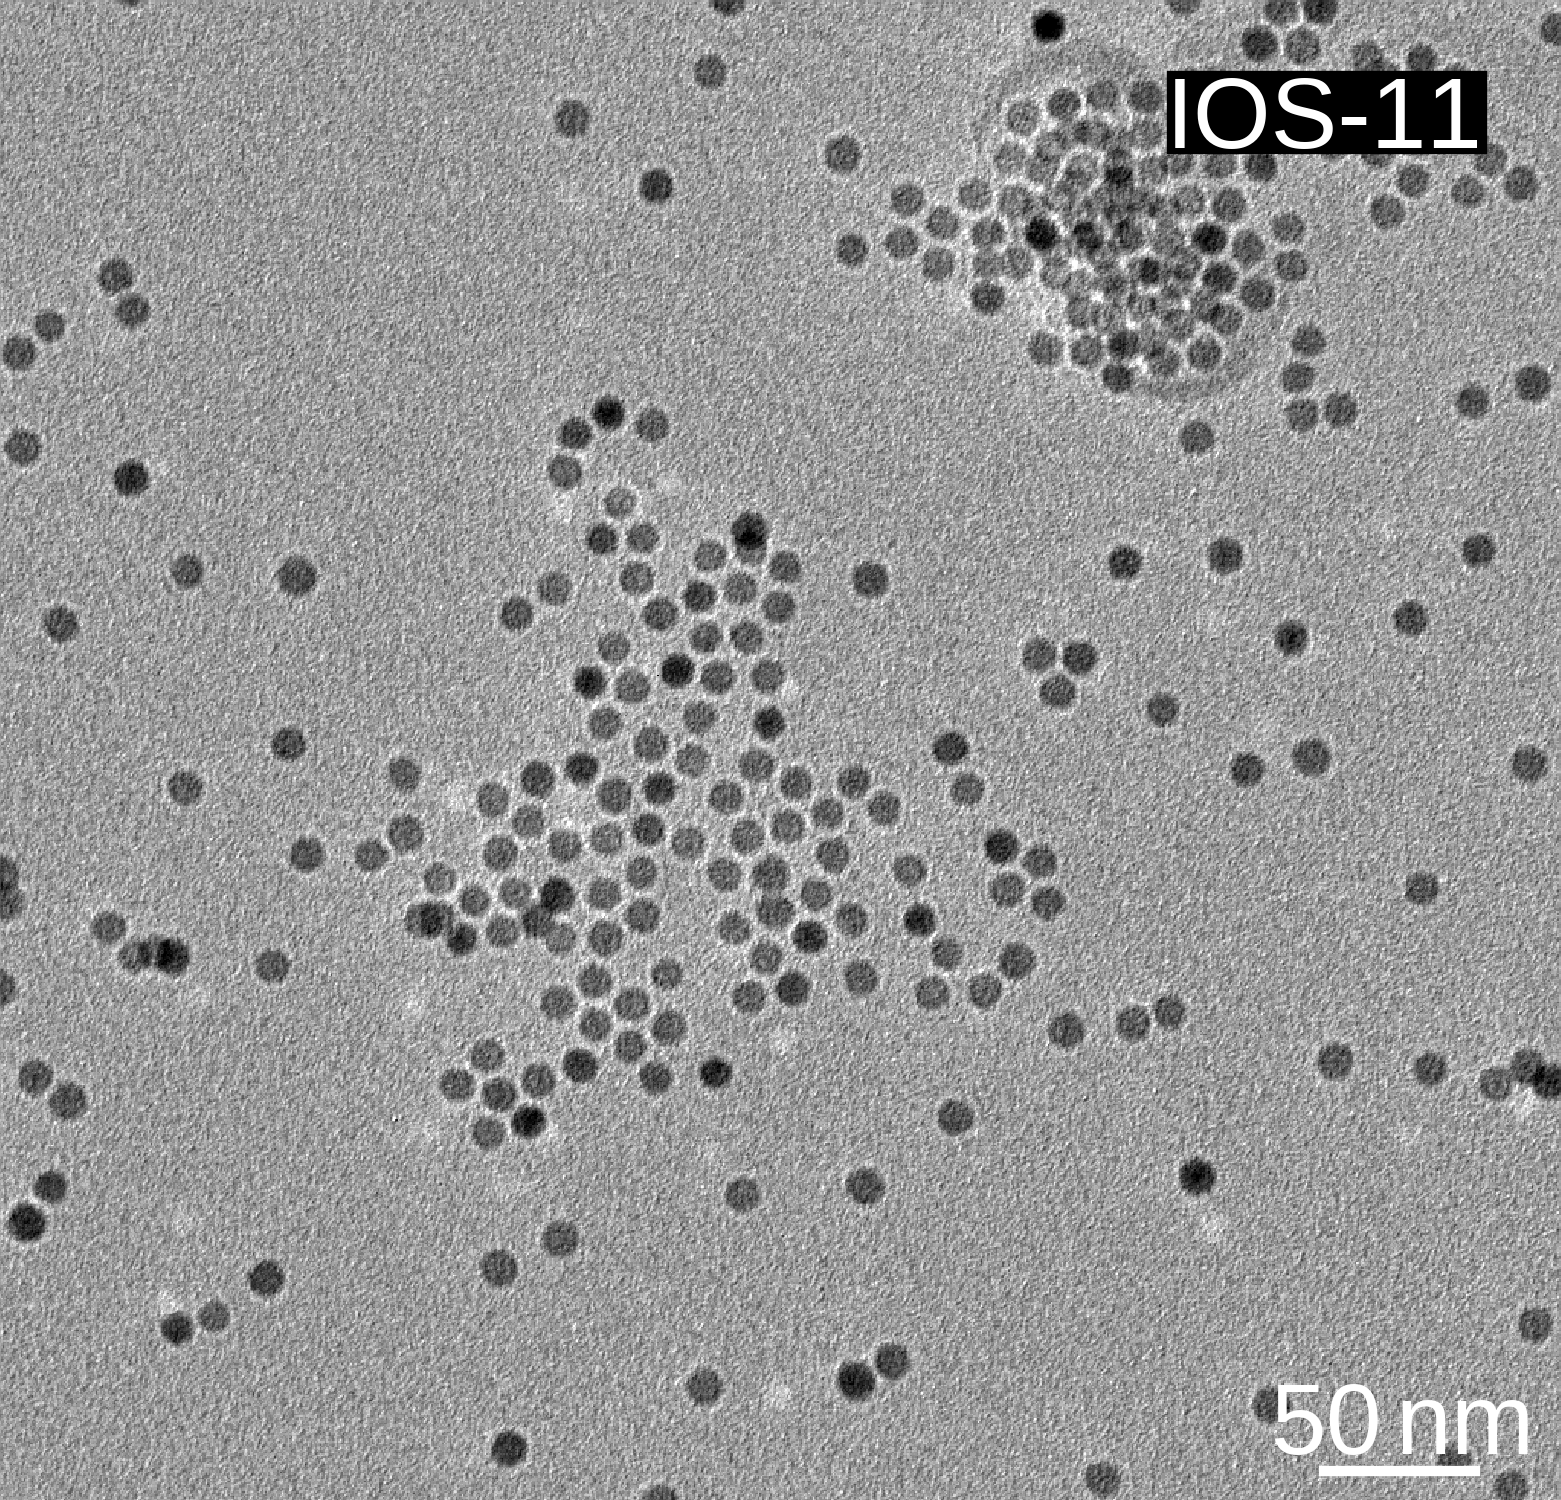
\includegraphics{looselyPackedNP_TEM_PMK18}
  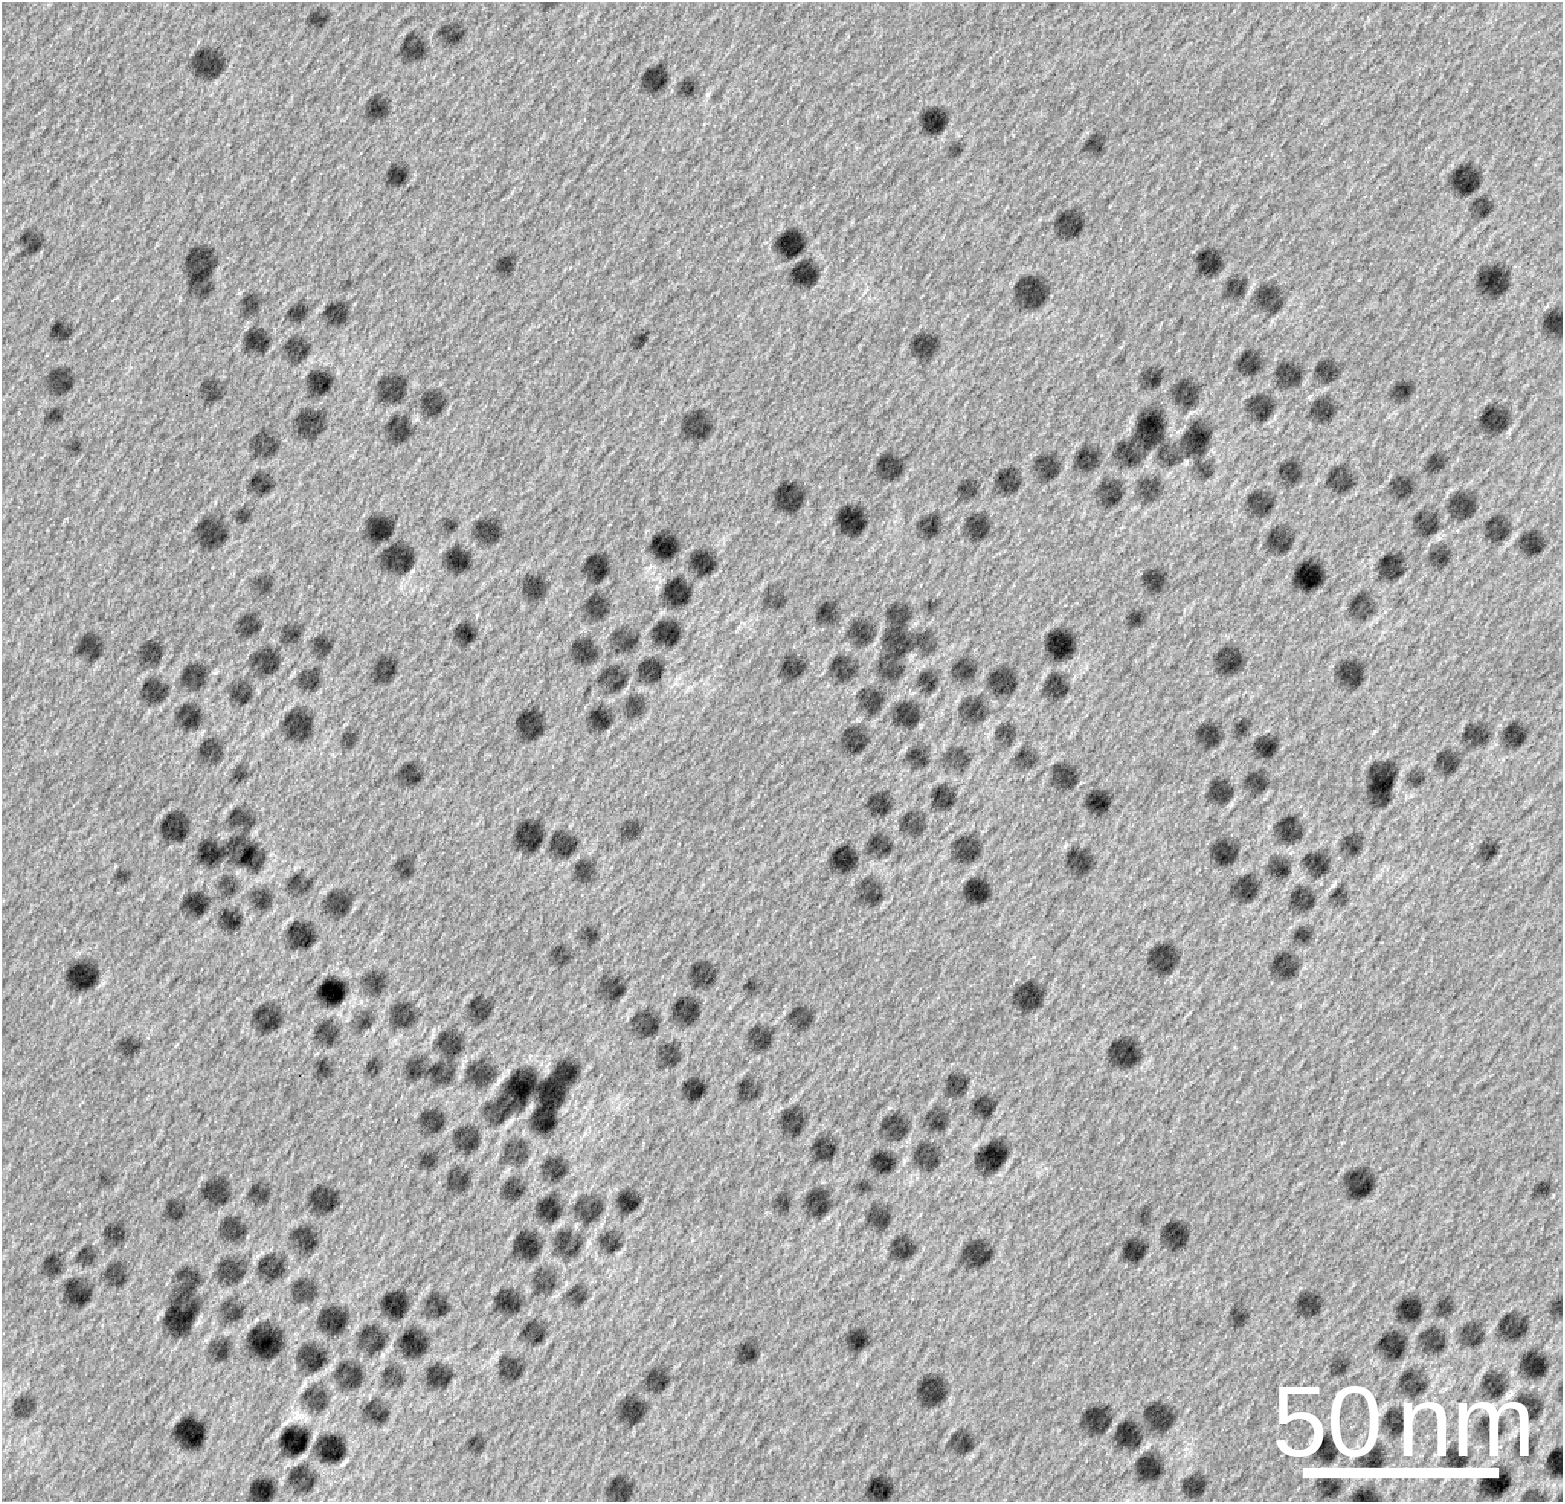
\includegraphics{looselyPackedNP_TEM_KWi338}
  \caption{\label{fig:looselyPackedNP:nanoparticle:tem}Transmission electron microscopy images of the $10 \unit{nm}$ (left) and $7 \unit{nm}$ (right) iron oxide nanospheres.}
\end{figure}

\section{Preparation of Monolayers}

\section{Nuclear Structure}

\section{Magnetic Structure}

\section{Emergent Effects}

\section{Model}

\end{document}